\subsection{Overlapping Periods}

The chains of parameter regions with the same period overlap.
We can see this in \Cref{fig:state.og.overlapping.chains}, which shows the boundaries of parameter regions with the same period.
Therefore, we can only see the boundaries of the chains and not all boundaries of the single parameter regions that make up the chain.
For \Cref{fig:state.og.overlapping.chains.full}, the fixed and varied parameters are the same as in previous 2D scans like \Cref{fig:state.og.dynamics.period}.
For the zoomed-in version \Cref{fig:state.og.overlapping.chains.zoomed}, the fixed parameters are the same but the varied parameters $E_0$ and $\chi_0$ are now in the ranges $[16.4, 17.2]$ and $[0.16, 0.22]$, respectively.

\begin{figure}
	\centering
	\begin{subfigure}{0.4\textwidth}
		\includegraphics[width=\textwidth]{99_Yunus/2D_Regions_Zoomed/result.png}
		\caption{Overview}
		\label{fig:state.og.overlapping.chains.full}
	\end{subfigure}
	\begin{subfigure}{0.4\textwidth}
		\includegraphics[width=\textwidth]{99_Yunus/2D_Regions_Zoomed2/result.png}
		\caption{Zoomed In}
		\label{fig:state.og.overlapping.chains.zoomed}
	\end{subfigure}
	\caption[2D scan of the boundaries of parameter regions with different periods in the original model]{
		2D scan of the boundaries of parameter regions with different periods in the original model.
		The parameters $\beta = 1, f = 150, L = 4.2 \cdot 10^{-3}, R = 2, V_m = 5,$ and $\mu = 0.5$ are fixed.
		In (a), the parameters $E_0$ and $\chi_0$ are varied in the ranges $[14, 28]$ and $[0.1, 0.65]$, respectively.
		(b) shows a zoomed-in version with the parameters $E_0$ and $\chi_0$ being varied in the ranges $[16.4, 17.2]$ and $[0.16, 0.22]$, respectively.
	}
	\label{fig:state.og.overlapping.chains}
\end{figure}

\Cref{fig:etup.og.overlapping.regions.zoomed} shows the boundaries of parameter regions with different symbolic sequences.
The fixed parameters and varied parameters are the same as in \Cref{fig:state.og.overlapping.chains.zoomed}.
This allows us to see the boundaries of the individual parameter regions that make up the chains.
And one can see, that the ``type A'' and ``type B'' parameter regions of the same chain also overlap.
\Citeauthor{akyuz2022} found in his thesis that there are 3 coexisting cycles in such an overlap.
One of the cycles is from the ``type A'' parameter region and the other 2 cycles are from the ``type B'' parameter region.

\begin{figure}
	\centering
	\includegraphics[width=0.6\textwidth]{98_Yunus_modpi/2D_Regions_Zoomed2/result.png}
	\caption[2D scan of the boundaries of parameter regions with different symbolic sequences in the original model]{
		2D scan of the boundaries of parameter regions with different symbolic sequences in the original model.
		The parameters $\beta = 1, f = 150, L = 4.2 \cdot 10^{-3}, R = 2, V_m = 5,$ and $\mu = 0.5$ are fixed.
		The parameter ranges of $E_0$ and $\chi_0$ are the same as in \Cref{fig:state.og.overlapping.chains.zoomed}, $[16.4, 17.2]$ and $[0.16, 0.22]$, respectively.
		Here, we can see the boundaries of ``type B'' parameter regions as they have different symbolic sequences as the neighboring ``type A'' parameter regions of the same chain.
	}
	\label{fig:etup.og.overlapping.regions.zoomed}
\end{figure}

The scans in this subsection are computed in the following way.
The program scans in 4 directions, from top to bottom (red), from bottom to top (blue), from left to right (yellow), and finally right to left (purple).
While scanning, it keeps track of the cycle it converged to last and marks the point, at which it loses the cycle.
This way, we can see where different parameter regions with cycles of different period overlap.

This also causes some errors in the diagrams, unfortunately.
When a scan starts in a parameter region where multiple cycles of different periods coexist, the cycle it sees at the first parameter point is determined by chance.
So for example two rows that scan from left to right and start in a parameter region where multiple stable cycles coexist might disagree on the period.
We can see this happening with the yellow lines in the lower left area of \Cref{fig:etup.og.overlapping.regions.zoomed}.
